\documentclass{rspublic}   

%------------------------------------------------------------------------- 
% take the % away on next line to produce the final camera-ready version 
\pagestyle{empty}

%\usepackage[utf8]{inputenc}
\usepackage{graphicx}
\usepackage{url}
\usepackage{float}
\usepackage{times}    
\usepackage{multirow}    
\usepackage{listings}   
\usepackage{times}     
\usepackage{paralist}    
\usepackage{wrapfig}    
\usepackage[small,it]{caption}
\usepackage{multirow}
\usepackage{ifpdf}    
              

%Bibliography                     
\usepackage{natbib}   

\usepackage{listings}
\usepackage{keyval}  
\usepackage{color}
\definecolor{listinggray}{gray}{0.95}
\definecolor{darkgray}{gray}{0.7}
\definecolor{commentgreen}{rgb}{0, 0.4, 0}
\definecolor{darkblue}{rgb}{0, 0, 0.4}
\definecolor{middleblue}{rgb}{0, 0, 0.7}
\definecolor{darkred}{rgb}{0.4, 0, 0}
\definecolor{brown}{rgb}{0.5, 0.5, 0}



\title[Adaptive Distributed Replica-Exchange Simulations]{Adaptive Distributed
  Replica-Exchange Simulations}

\author[Luckow, Jha, Kim, Merzky, Schnor]{
  Andre Luckow$^{1}$, Shantenu Jha$^{2,3,4}$, Joohyun Kim$^{2}$, Andre Merzky$^{2}$ and Bettina Schnor$^{1}$\\
  \small{\emph{$^{1}$Institute of Computer Science, Potsdam University, Germany}}\\
  \small{\emph{$^{2}$Center for Computation \& Technology, Louisiana State University, USA}}\\
  \small{\emph{$^{3}$Department of Computer Science, Louisiana State
      University, USA}}\\
  \small{\emph{$^{4}$e-Science Institute, Edinburgh, UK}}\\
}

%\date{}

\def\acknowledgementname{Acknowledgements}
\newenvironment{acknowledgement}%
{\section*{\acknowledgementname}%
\parindent=0pt%
}


\newcommand{\I}[1]{\textit{#1}}
\newcommand{\B}[1]{\textbf{#1}}
\newcommand{\T}[1]{\texttt{#1}}

\newcommand{\glidein}[1]{Glide-In }  
\newcommand{\replicaagent}[1]{Replica-Agent }         
\newcommand{\remanager}[1]{RE-Manager }

\begin{document} 

\maketitle    


\begin{abstract}{Replica-Exchange, SAGA, Migol, Adaptive, Fault-Tolerance}  
  Due to the loose-coupling between replicas, the Replica-Exchange
  class of algorithms should be able to benefit greatly from utilising
  as many resources as available. However, the ability to effectively
  utilise multiple distributed resources to reduce the
  time-to-com\-ple\-tion remains a challenge at many levels.
  Additionally, an implementation of a {\it pleasingly-distributed}
  algorithm such as Replica-Exchange, which is independent of
  infrastructural details does not exist.  This paper proposes an
  extensible and scalable framework based on SAGA that provides a
  general-purpose, opportunistic mechanism to effectively utilise
  multiple resources in an infrastructure independent way. By
  analysing the requirements of the Replica-Exchange algorithm and the
  challenges of implementing it on real production systems, we propose
  a new abstraction (BigJob), which forms the basis of the adaptive
  redistribution and effective scheduling of replicas.
\end{abstract}

\section{Introduction}

Several classes of applications are well suited for distributed
environments. Probably the best known and most powerful examples are
those that involve an ensemble of decoupled tasks, such as simple
parameter sweep applications~\citep{1239909}.  A slightly more
complicated and challenging class of distributed applications are
those that have a degree of coupling between individual sub-tasks.  An
interesting example of such applications are those based upon the
\emph{Replica-Exchange (RE)}~\citep{hansmann,Sugita:1999rm} algorithm.
RE simulations are used to understand physical phenomena -- ranging
from protein folding dynamics to binding affinity calculations.

%%%%% RE nature of the problem
The RE method involves the concurrent execution of multiple similar
simulations -- the \emph{replicas}. The coupling between the replicas
occurs via periodic exchange attempts between paired replicas. The
exchange is typically infrequent compared to the run-time of each
replica, and is small in terms of communication bandwidth
requirements. Thus, RE is {\it prima facie} a perfect algorithm to
exploit distributed resources. We label such a class of algorithms as
{\it pleasingly-distributed}.

%%%%% related work
Most RE implementations are either infrastructure
specific~\citep{Woods:2005nx}, or if using multiple distributed
resources, require prior co-scheduling~\citep{repex_mpig}.
Ref.~\citep{repex_mpig} is an important example of a first-generation
Grid application, wherein the effectiveness of coupling multiple
distributed resources for scientific problems has been demonstrated.
The real power of distributed systems however, arises from adaptive
algorithms and implementations that provide applications with an agile
execution model, and thus the ability to utilise resources
dynamically, as opposed to a static execution model inherited from
parallel and cluster computing.  Unfortunately, the barrier to the
development of such adaptive applications is high and the
infrastructure support is poor.
Specifically, there is no implementation of an
adaptive RE algorithm, which is both able to effectively and reliably
utilise multiple distributed resources without prior scheduling as
well as being independent of any specific %computational platform or
infrastructure.

In this paper we address some of the challenges and performance
bottlenecks encountered when performing RE simulations over multiple
distributed resources, such as the overall slowdown due to
synchronisation arising from the light-coupling and the lack of
co-scheduled resources.  The unique contribution of this paper is the
implementation of a RE framework that overcomes the described
limitations by being able to adapt at runtime to a change in the
availability of resources and application resource requirements.  The
framework builds upon preliminary work of integrating SAGA and Migol to
provide fault-tolerance.
While SAGA represents a well-defined, standardized interface for writing
Grid applications, Migol provides the underlying middleware services
to guarantee the correct and reliable exe\-cution of applications even
in the presence of failures~\citep{Luckow:2008la}.

We provide evidence that, as more resources become
available, our framework can opportunistically utilise these resources,
leading to a reduction in the time-to-completion of the scientific
problem.  The remainder of the paper is structured as follows: In the
next section we provide the basic ideas and advantages of using RE
simulations to understand physical properties of a RNA system. In
section~\ref{sec:remd_impl} we describe the details of the REMD
framework implementation. Section~\ref{sec:glidein} discusses the new BigJob
abstraction and the SAGA Glide-In framework.  
In section 5 we describe the deployment and results of different experiments
using the SAGA based RE framework on the TeraGrid, and in section 6 we
present data establishing the advantages of REMD for the physical
system under study. 


\section{Hepatatis-C Virus (RNA) Using Replica-Exchange}

In Molecular Dynamics (MD) approaches, sufficient sampling of
configurations is an important requirement for connecting atomistic
results to macroscopic or thermodynamic quantities available from
experiments. This provides an important motivation for researching ways 
to accelerate sampling and to enhance the ``effective''
time-scales studied. 
Generalized ensemble approaches -- of which
REMD~\citep{Sugita:1999rm} is a prominent example -- represent a
% important and 
promising attempt to overcome the general limitations of
insufficient time-scales, as well as specific limitations of
inadequate conformational sampling arising from kinetic trappings.
The fact that one single long-running simulation can be substituted
for an ensemble of loosely-coupled shorter-running simulations, make
these ideal candidates for distributed environments.

RE simulations consist of
two distinct components: the underlying simulation engine
used for each replica, and the coupling-mechanism between the
individual replicas.  
The degree and frequency of coupling and exchange can be either
regular~\citep{Sugita:1999rm}, or irregular~\citep{SPdynamics}. 
An example of the latter -- parallel replica dynamics as 
implemented in Folding@home
\citep{folding} involves coordination between replicas only when an
``event'' occurs.  In contrast, for regular RE applications, attempts
to exchange states between certain pairs occur at fixed intervals. 


The hepatitis C virus (HCV) internal ribosome entry site (IRES) is
recognized specifically by the small ribosomal subunit and eukaryotic
initiation factor 3 (eIF3) before viral translation initiation.  This
makes it a good candidate for new drugs targeting Hepatitis-C virus.
Our aim is to use REMD to enhance the sampling of the conformational
flexibility of the internal loop referred to as {\it HCV IRES IIIb CA
  variant}~\citep{Collier:2002wd} as well as the equilibrium
energetics.  The model of the physical system under investigation in
this work is comprised of a RNA system of nucleotides; the total
number of atoms in the simulating box is 21887 -- including the RNA
system, explicit water molecules, and ions for neutralization of the
system.  The initial conformation of the RNA is taken from the NMR
structure (PDB ID: 1PK7).


\section{Implementing Distributed Replica-Exchange Using SAGA/Migol}
\label{sec:remd_impl}

{\it \bf RE-Manager Architecture:} The
framework comprises of three components, the RE-Man\-ag\-er,
the Replica-Agent and the Migol infrastructure. 
The  \emph{RE-Manager}, also referred to as task manager,
is deployed on the user's desktop and provides the interface 
to the overall RE run. It orchestrates all replicas, which involves
file staging, job spawning and the conduction of the 
exchange attempts, using the SAGA APIs.                                                                

The second element is the task agent, the \textit{Replica-Agent},
that resides on the machines where the RE replicas
are executed. The \replicaagent\ is launched using SAGA CPR and Migol.
%It is responsible for spawning and monitoring of the replicas. 
NAMD~\citep{Phillips:2005gd}, a highly scalable, parallel MD code, is
used to carry out the MD simulation corresponding to each replica
run. It is important to mention that any other MD or
Monte Carlo code could be used just as simply and effectively.
Finally, Migol handles the reliable execution of the Replica-Agent and
the replicas, i.\,e.\ the submission, the monitoring and, 
if required, the recovery of replicas or the application itself.

                       
\noindent                                            
{\it \bf Replica-Exchange Logic:} RE simulations involve the running 
of multiple replica jobs.
% to enhance the sampling of configuration space. In the case of REMD 
Each replica is assigned a different temperature.  Depending on the number of
processes $n$, the \remanager\ creates $\frac{n}{2}$ pairs
of replicas.  Before launching a job the \remanager\ ensures that all
required input files are transferred to the respective resource. For
this purpose, the SAGA File API and the GridFTP adaptor are used.  
The replica jobs are then submitted to the resource using the SAGA CPR API and
the Migol/GRAM middleware. 

When all replicas reach a pre-determined state (e.\,g. the NAMD job
finishes after a fixed number of steps), the decision as to whether to
pairwise exchange temperatures between neighbouring replicas is
determined by the Metropolis scheme.  
The run of an ensemble of replicas
in parallel and the subsequent pairwise exchange attempt 
is referred to as \emph{generation}. No two replicas can belong to
different generations.  If the exchange attempt is successful, parameters such as the
temperature, are swapped. Both jobs are then relaunched. 
%using the mechanisms described above. 
Often the Metropolis scheme returns a
negative result, and an exchange is not carried out; thus it is
difficult to respond to a possible exchange speculatively.


\noindent
{\it \bf Deploying on Production Environments:} The RE framework has 
been successfully deployed on LONI and TeraGrid production 
resources~\citep{Luckow:2008la}. In these environments a significant
slowdown was observable, in particular when running a larger number
of replicas.
A major reason for this slowdown was the fact that
the re-started replicas are required to queue again at
the local scheduler.  In pathological cases, the complete system 
came to a halt solely due to a single crowded or slow resource.

To avoid such bottlenecks, the multiple sub-tasks that comprise
distributed applications need to avoid re-queuing at the system
batch-queue level.  Additionally, distributed applications that are
decomposable into sub-tasks should be able to respond to the dynamic
availability of resources.  Unfortunately, current infrastructures do
not support such dynamic scheduling directly. To provide
this capability to applications, we need (i) abstractions that enable
agile execution models via application-level allocation of resources,
and (ii) different adaptivity strategies that determine how resources
are efficiently utilised.  {\it The following section describes the
  extensions to the simple RE framework that enables efficient
  scheduling of sub-tasks and supports adaptive applications.}

\vspace{-0.15in}
\section{Adaptive Replica-Exchange: Abstractions and Implementation}
\label{sec:glidein}

As motivated before, the use of multiple {\it simple} Grid jobs to
execute many replicas has a severe limitation: all simple jobs must
queue at the resource management system, i.\,e.\ a single delayed
job can cause an overall slowdown.  We overcome
this issue by using an efficient dispatching scheme, which builds upon
the ability to cluster replicas using the novel BigJob abstraction
before submission. Based on this abstraction, we propose different
strategies that address the dynamic conditions of distributed
environments.


{\noindent \it \bf Abstractions:} A common approach to
avoid queuing delays is the use of place-holder jobs, which are
able to dispatch several sub-jobs without each sub-job needing to
queue at the local scheduler. A specific mechanism to support this
pattern is the \emph{Glide-In} abstraction, in reference to the Condor
Glide-In system~\citep{citeulike:291860}, which pioneered this idea. A
Glide-In job requests a sufficiently large chunk of resources; smaller
sub-jobs can then rapidly be executed through the Glide-In job.  By
avoiding the high initial costs for queueing each individual replica
job, the time-to-completion can be dramatically reduced.

\begin{figure}[t]
    \begin{center}  
      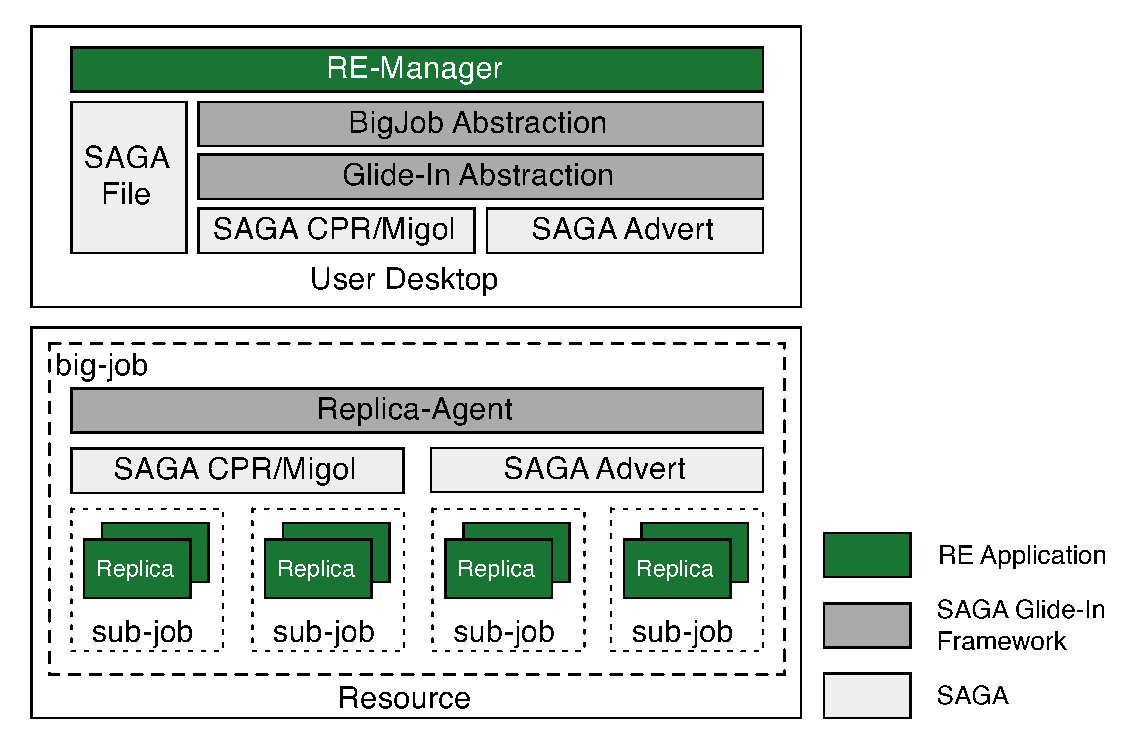
\includegraphics[width=0.67\textwidth]{remdmanager_v12}
      \caption{\footnotesize \bf RE-Manager Abstractions: The BigJob
          abstraction provides the capability to cluster sub-jobs into a
          larger big-job, and is implemented on top of the Glide-In
          abstraction.\vspace*{-3em}}
     \label{fig:abstractions} 
    \end{center}
\end{figure}

Figure~\ref{fig:abstractions} summarizes the abstractions developed
and used in this work to support the clustering of sub-jobs into 
larger big-jobs and the effective dispatching of the sub-jobs.  The
specific capability to cluster sub-jobs, is provided to the
application via the \emph{BigJob} abstraction. 
The SAGA Glide-In abstraction is used to
support the commonly occurring place-holder job pattern.
The BigJob abstraction defines a \texttt{big\_job}
and \texttt{sub\_job} object; for each \texttt{big\_job}
object, a Glide-In job with the desired number of resources is
started, and \texttt{sub\_job} objects, which correspond to
individual replicas, are mapped to a \texttt{big\_job} using the jobid
as reference. It is helpful to reiterate that although there is a
\texttt{big\_job} object, it is submitted as a Glide-In job. Also, the
BigJob abstraction in turn utilises the Glide-In abstraction to map the
individual big-job and sub-jobs to physical resources.

\begin{figure}[t]
	    \begin{center}  
	      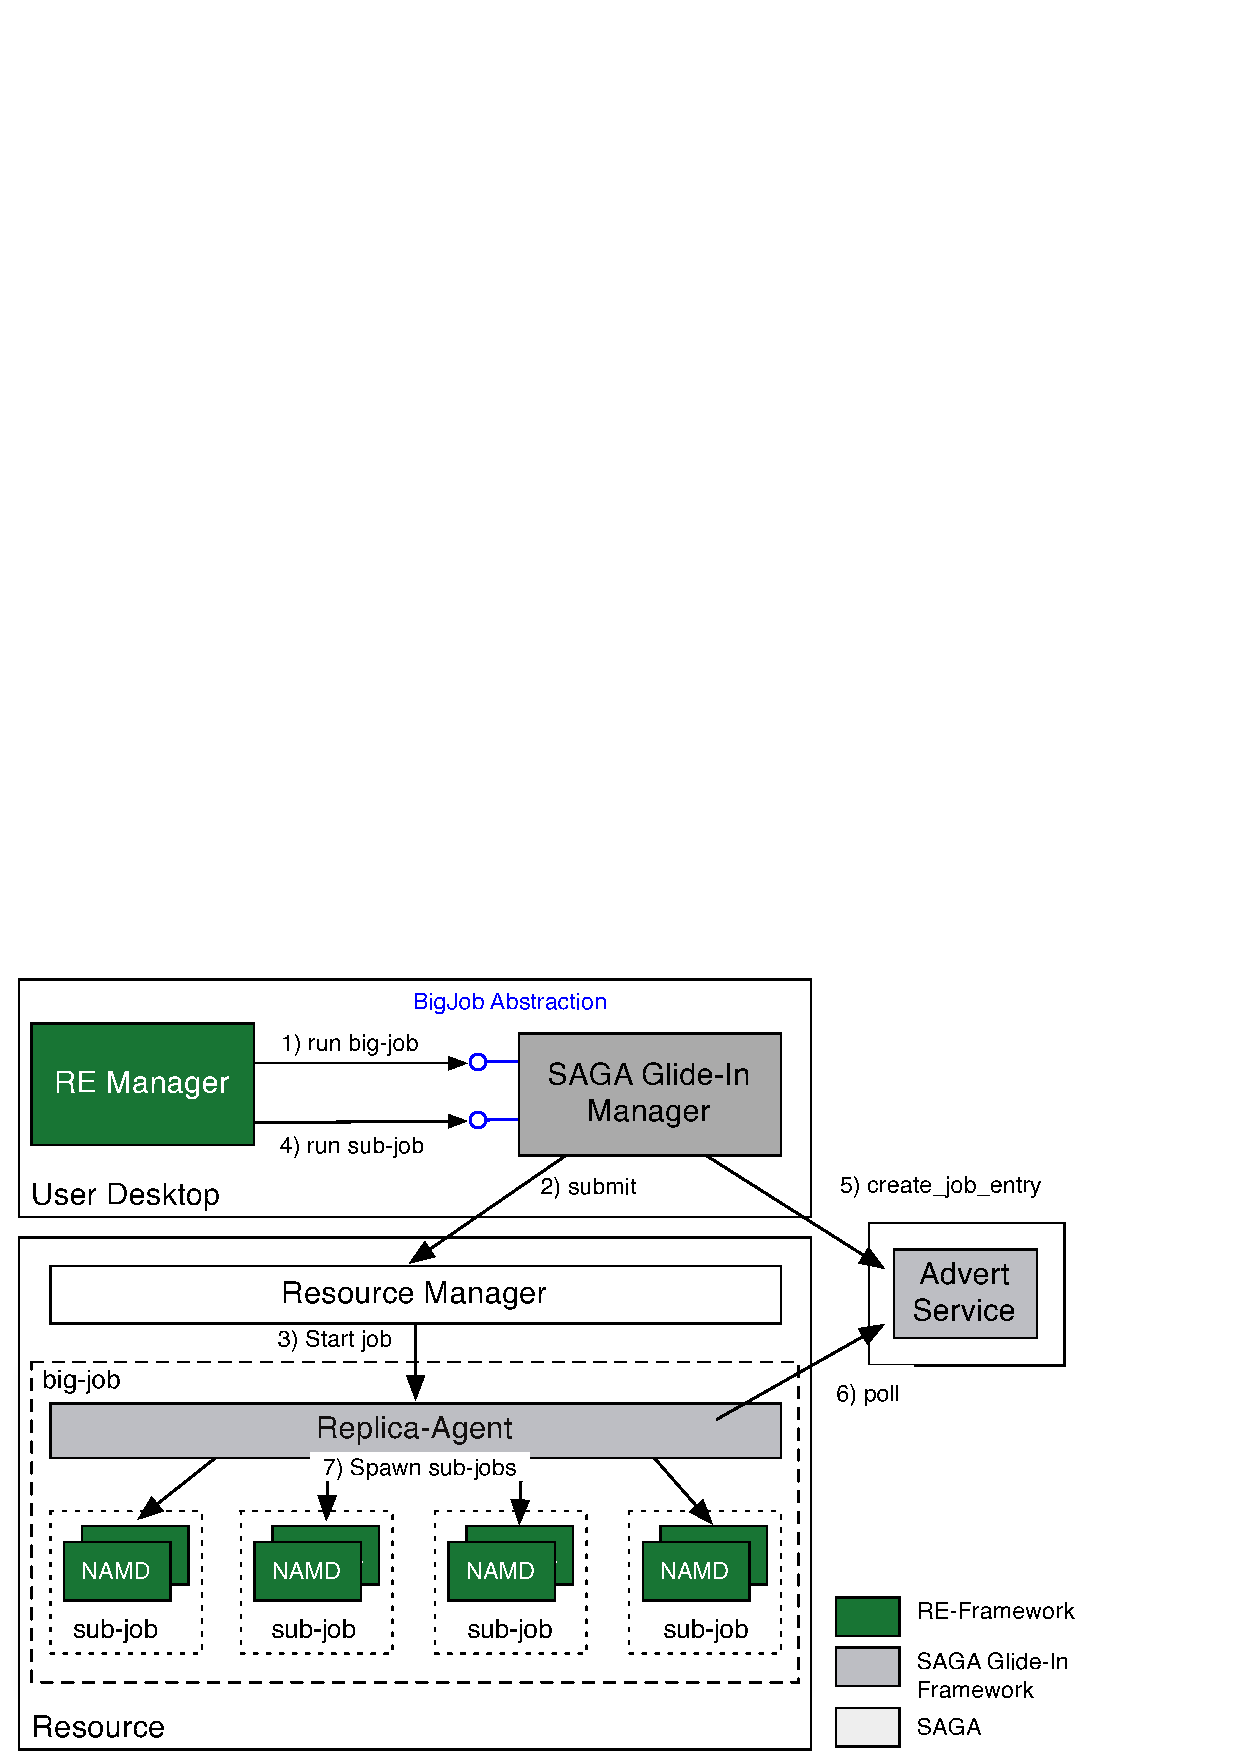
\includegraphics[width=0.67\textwidth]{re_bigjob_interactions_v2}
	      \caption{\footnotesize \bf RE-Manager and SAGA-Glide-In Framework:
	        The Glide-In job (Replica-Agent) is used as place-holder job
	        for all replica sub-jobs running on a single cluster. The
	        \remanager\ can control both the \replicaagent\ and the replica
	        jobs.\vspace*{-1em}}
	        \label{fig:remdmanager_v1.1}   
	    \end{center}
\end{figure}

{\noindent \it \bf Implementation:} The RE framework has been
extended to support the BigJob and Glide-In abstractions.
BigJob provides the ability to cluster sub-jobs; Glide-In allows the
effective scheduling of the sub-jobs.  As illustrated in
Figure~\ref{fig:remdmanager_v1.1}, the RE-Manager uses the
\texttt{big\_job} and \texttt{sub\_job} objects as replacements for the
\texttt{job} object defined by SAGA CPR.  The \texttt{big\_job} and
\texttt{sub\_job} objects behave similarly to regular SAGA CPR job
objects. Thus, the RE-Manager, which is the application in this case,
does not require any extensive modification; 
all that the RE-Manager has to do is to provide a mapping 
from a \texttt{sub\_job} to a suitable \texttt{big\_job} via a jobid.

% BigJob
The SAGA Glide-In implementation comprises of three components: 1) The
\emph{Glide-In Manager}, which provides the Glide-In abstraction and
manages the orchestration and scheduling 
of Glide-In jobs (which in turn allows
the management of both big-job objects and sub-jobs) and 2) The
\emph{Replica-Agent}, which represents the Glide-In job and thus, the
application-level resource manager on the respective resource, and 3)
the \emph{Advert Service}, which is used for communication between the
Glide-In Manager and Replica-Agent.


Before running regular jobs, an application, in this case the 
RE-Manager, must initialize a \texttt{big\_job} object. 
The Glide-In Manager then queues a Glide-In
job, which actually runs a Replica-Agent on the respective resource.  
For this \texttt{big\_job} instance the
specified number of resources is requested. Subsequently,
\texttt{sub\_job} objects can be submitted through the Glide-In
Manager using the jobid of the \texttt{big\_job} as reference.
The Glide-In Manager ensures that the sub-jobs are launched onto the 
correct resource based upon the specified jobid using the right number
of processes.

Communication between the Replica-Agent and Glide-In Manager is
carried out using the SAGA Advert Service, a central key/value
store. For each new job an advert entry is created by the
Glide-In Manager. The \replicaagent\ periodically polls for new jobs.  If a
new job is found and resources are available, the job is dispatched, 
otherwise it is queued. Further, the agent encapsulates
local machine-specific settings. The \replicaagent\
ensures e.\,g.\ that the right combination of compiler, MPI library and NAMD
executable is used.


{\noindent \it \bf Adaptive Replica Scheduling:} Distributed applications
including RE simulations must be able to deal with time-varying
resource availabilities.  An application is referred to as
\emph{dynamic} when either its resource requirements, 
or the availability and utilisation of resources 
changes during its runtime.  \emph{Adaptivity} is a
mechanism to respond to dynamic
changes; % as opposed to just ignoring the dynamism of a distributedenvironment.
a dynamic application may deploy multiple adaptive strategies or
choose between competing adaptive strategies.  For an application to
be adaptive, it is necessary for it to be able to effectively
utilise an expanded or reduced set of resources; additionally for an
adaptive application to be scalable it must also be able to
determine which resources to utilise efficiently.
For resource determination, our framework currently relies on a
static, user-defined mapping of replicas and resources.  In the
remainder of this paper, we will focus on dynamic resource
utilisation (and not on dynamic resource determination or
optimisation).

For jobs that want to maximise their throughput the ability to adapt
to dynamically changing resource loads is critical. 
It is equally important for long-running applications to be
able to support an agile execution model allowing the effective
utilisation of resources as they become available.  Specifically,
there are different ways a RE simulation can respond to a change in
the number of resources required/available:
\begin{compactitem}         
\item {\it Scenario A:} By increasing the number of processes assigned
  to each replica the time-to-completion can be reduced. In addition,
  resources can be partitioned in a way that balances the different
  speeds of resources.  For example, by adding processes to a 
  delayed replica, bottlenecks due to synchronisation of replicas can
  be avoided.

\item {\it Scenario B:} As resources become available, the
  number of replicas can be adjusted. Depending on the underlying
  physics model, the additional replicas can be used to either refine
  the temperature range (adaptive sampling) or to extend the
  temperature range (enhanced dynamics). This REMD approach is also
  referred to as \emph{Cool Walking}~\citep{coolwalking}.
\end{compactitem}           
Our framework supports both adaptive strategies.


\section{Distributed Replica-Exchange on the TeraGrid}
\label{sec:exp}
        
To evaluate the performance of the RE-Manager several experiments have
been conducted on TeraGrid (TG) and LONI resources. The resources
used are: Ranger (TG), Abe (TG) and QueenBee (QB; both TG and LONI).
% We investigated the performance of the SAGA Glide-In mechanism under
% different adaptivity modes.  
The RE-Manager was configured to run a parallel NAMD simulation with up to 16
replicas sampling a temperature range between 300 and 450\,K. Replica
exchanges are carried out between pairs of replicas. Thus,
there are up to 8 exchanges in each generation. Each test run comprises
of up to 64 attempted exchanges; each replica can 
use up to 24 MPI processes and runs for 500 time steps 
between exchange attempts. The metric used 
is the time-to-completion for 64 attempted exchanges.

Initially, we investigated the effect of the 
Glide-In framework on the time-to-completion ($T_{c}$) using 16
replicas on QB.  Using the Glide-In framework, there was a reduction
in $T_{c}$ from 52\,minutes to 26 minutes per average, which
corresponds to a decrease of 50\,\%.  In the best case,
improvements of up to 70\,\% were observed. This effect
is attributed to the elimination of the queuing times for every
sub-job. Once the Replica-Agents become active, replicas can be
dispatched without requiring interactions with the local
scheduler.

Further, we performed tests for the two adaptive scenarios.
In the scenario A, the number of replicas was kept constant
(Conventional REMD) and the \emph{replica size}, i.\,e.\ the number of
MPI processes assigned to each replica was varied as more resources
became available.  In scenario B, the \emph{replica number}, i.\,e.\ the
number of replicas participating in a generation, was varied (Cool
Walking).  We compare $T_{c}$ for 64 attempted exchanges on different sets of
distributed resources and Glide-In configurations.
                    
\begin{figure}[h]
  \begin{minipage}[t]{.48\textwidth}
    \begin{center}  
      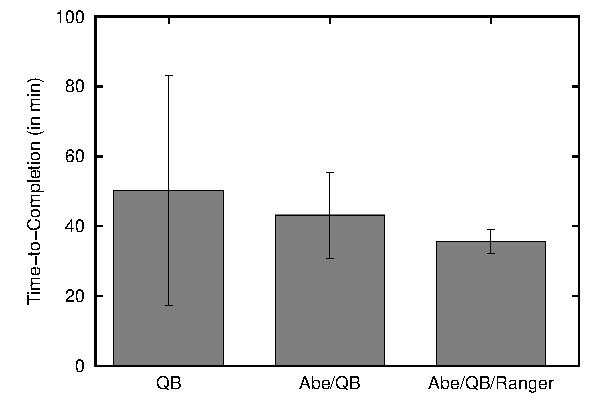
\includegraphics[width=\textwidth]{perf_distributed_size_replica}
      \caption{\footnotesize \bf Replica Size Adaptivity (Scenario A):
        As the number of resources available increases, the number of
        cores assigned to a replica (a NAMD job) is dynamically
        adjusted, while keeping the number of replicas constant at
        sixteen.  There are 4~Glide-Ins with 32 cores each.  
        As more resources become available, more cores are
        assigned to each replica, which leads to a reduction
        of $T_{c}$.  }
      \label{fig:performance_perf_distributed_A}
    \end{center}
  \end{minipage}
  \hfill
  \begin{minipage}[t]{.485\textwidth}
    \begin{center}  
      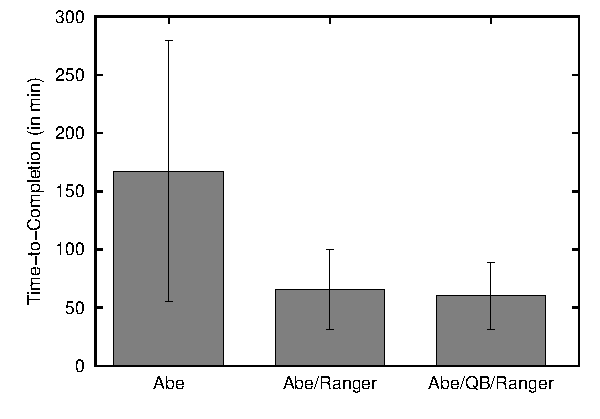
\includegraphics[width=\textwidth]{perf_distributed_number_replica}
      \caption{\footnotesize \bf Replica Number Adaptivity (Scenario
        B): In this scenario, the framework dynamically adjusts the
        number of replicas.  A constant number of 4 Glide-Ins with 64
        cores each are distributed across 1, 2 and 3 machines; the
        size of each replica is kept fixed at 16 cores. Once again,
        the greater the number of distributed resources that can be
        utilised, the smaller $T_{c}$.}
      \label{fig:performance_perf_distributed_B}
    \end{center}
  \end{minipage}
  \hfill
\end{figure}

In scenario A, up to 3 different resources are used, the number of
Glide-Ins varies from 4 up to 12, whilst the number of replicas used is
fixed at 16. Thus, the size of the individual replicas is varied.
When a resource is being used, it runs 4 Glide-Ins and each Glide-In
job has a constant size of 32 cores.  Although, the number of
Glide-In jobs on a resource is fixed at 4 for reasons of simplicity,
our results will hold for general values. If all
resources (Abe, QB and Ranger) were being used, there would be 12
Glide-In jobs with 32 cores each, i.\,e.\ a total of 384 cores would 
be available.  Glide-Ins
are submitted to 1, 2 or 3 statically configured resources. After submission
the Glide-Ins are subject to different queueing delays at the local
schedulers. To reflect these different loads, the number of
MPI processes assigned to each replica is dynamically
increased as new resources become available.
% (and therefore the number of Glide-Ins can be increased). 
Depending on the number of available
resources, between 8 (for 4 Glide-Ins) and 24 MPI processes (for 12 Glide-Ins)
are used for each replica.

Figure~\ref{fig:performance_perf_distributed_A} shows the results of
the distributed run. In spite of the overhead for migrating replicas
to newly available resources, a notable decrease in $T_c$ of up to
15\,minutes can be observed as the number of resources increases from
one to three. Although, the efficiency, defined as runtime on one
resource divided by the runtime on multiple resources scaled by the
number of resources, is only about 0.5, this is a limitation of the
used setup rather than a general scalability barrier.  The setup
comprises of rather short NAMD jobs; in particular during the initial
phase jobs are often migrated to other resources, which mainly causes
this overhead. During longer runs this overhead is 
negligible. What is also very important to note is the reduced
fluctuation in the $T_c$ when multiple resources are used. This is
indicative of the fact that there is a reduction in the sensitivity to
queue-loads -- something that applications on real production
environments have to battle with.  

% general setup
In scenario B, the capability of the RE-Manager to adaptively adjust
the number of replicas by varying either the
range of temperature or the specific temperatures simulated is
evaluated.  For this scenario, 4 Glide-Ins with 64 cores each
are distributed across either 1, 2 or 3 different distributed
resources. That means that the total of 256 cores is allocated on (i)
Abe only, (ii) Abe and Ranger (iii) Abe, Ranger and QB.
Each replica has a constant number of 16 MPI processes, and thus any
Glide-In can run exactly 4 replicas when active.

%  procedure
At the beginning of the experiment, all 4 Glide-Ins are submitted to
either 1, 2 or 3 resources (statically configured).  Similar to
scenario A, different queueing delays usually occur.
%; this is true whether using 1 resource or using 3.  
Consequently, not all Glide-Ins start
simultaneously.  Using the adaptive temperature sampling algorithm,
the number of replicas is dynamically varied as the number of active
Glide-Ins increases. Depending on the number of running Glide-Ins, the
ensemble consists of 4 to 16 replicas (increase in
steps of 4).


As shown in Figure~\ref{fig:performance_perf_distributed_B}, $T_{c}$
decreases with the number of resources used.  With the the simulation
distributed onto greater number of resources, the probability that a
single heavily-utilised resource delays the overall progress of the
simulation is reduced.
The results clearly demonstrate the benefits of the adaptive replica
scheme -- it is favourable to instantly use resources as they become
active instead of waiting for the complete set of nodes to become
available.  

\section{Results: Enhanced Sampling of Hepatitis-C Virus}
In the previous sections we discussed the design and performance of
the framework and showed how it enables the effective utilisation of
multiple resources. In section 2, we provided motivation for why the
RE approach is required to understand the energetics and
conformational flexibility of the internal loop of the Hepatitis-C
virus. The effectiveness of the RE approach in increasing the rate of
convergence to equilibrium (Boltzmann distribution) or enhancing the
sampling can be measured by the rate of attempted
exchanges~\citep{Lei:2007xe}, or equally by the inverse of the {\it
  time} between attempted exchanges.


REMD simulations (Scenario A) were performed for HCV IRES IIIb CA
variant using the model described in section 2. The replicas covered a
temperature range from 300\,K to 450\,K, thus fixing the number of
replicas to 16.  To demonstrate the effectiveness of our RE framework,
we analyse a typical time-series of the number of resources used
(available) and thus, the number of active Glide-Ins during a six hour
run on a production infrastructure.  Each Glide-In has 32 cores; 
thus, the number of cores for each replica is determined by the numbers of
active Glide-In jobs.  Figure~\ref{fig:result_A} shows how the number
of active Glide-Ins changed during the six hour interval. To start
with, there were only enough processors to support one Glide-In job,
but after approximately two hours, there were enough to activate two
Glide-Ins; after three hours three Glide-Ins are running. 
Eight Glide-Ins were activated before the six hour time
limit. As the number of Glide-Ins increases, the number of processors
assigned to each replica increases, with the physically important
consequence that there is a concomitant decrease in the average time
between exchange attempts (upper line in Figure~\ref{fig:result_A}).
The average time between exchange attempts as a function of the number
of active Glide-Ins and
the speedup -- measured as the inverse of the average time
normalised by the time taken with one Glide-In (thus the value of 1
for the one Glide-In case)  -- are shown in Figure~\ref{fig:result_B}.

\begin{figure}[h]
  \begin{minipage}[t]{.495\textwidth}
    \begin{center}  
      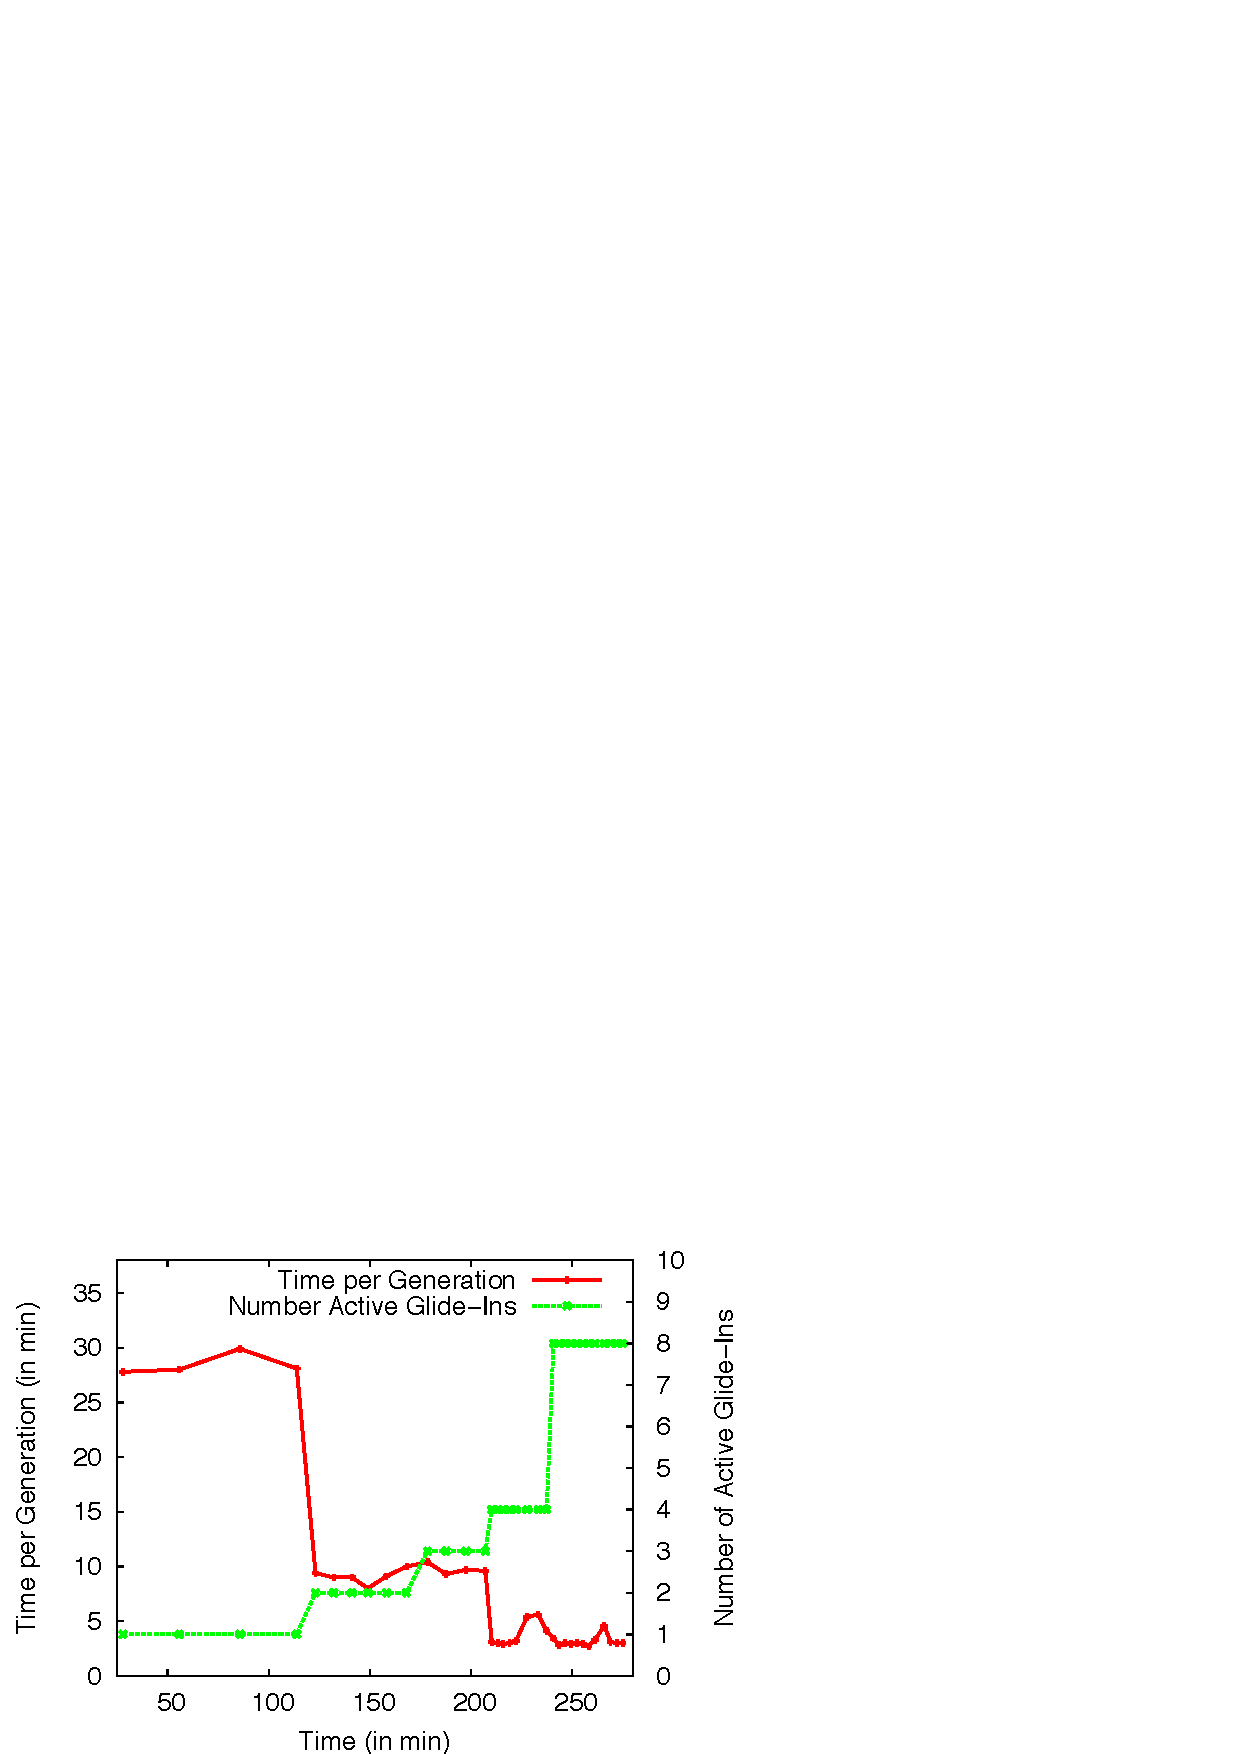
\includegraphics[width=\textwidth]{perf_repex}
      \caption{\footnotesize \bf The plots show the time-series of the
        average times between exchange attempts (upper line using the
        left-hand y axis) and the number of active Glide-Ins over a
        six-hour run on the TeraGrid.}
      \label{fig:result_A}
    \end{center}
  \end{minipage}
  \hfill
  \begin{minipage}[t]{.48\textwidth}
    \begin{center}  
     % \includegraphics[width=\textwidth]{}
      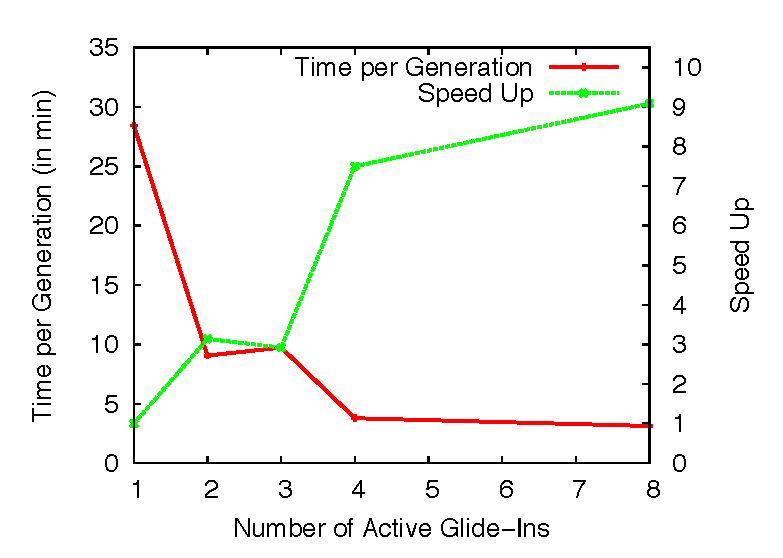
\includegraphics[width=\textwidth]{perf_repex2}
      \caption{\footnotesize \bf The upper plot (using the left-hand
        y axis) illustrates how the average time between exchange attempts
        decreases as the number of Glide-Ins increases. At the same time
        the speedup grows.}
        % The plot in        green shows the speedup.}
      \label{fig:result_B}
    \end{center}
  \end{minipage}
  \hfill
\end{figure}             


%% ----------------------------------------------------------------------------
\section{Conclusion and Future Work}

In summary, SAGA provides a well-defined and sufficiently powerful
interface to develop the required abstraction to support adaptive
distributed RE applications.  SAGA allows the simple decoupling
of the RE orchestration logic from the underlying distributed
infrastructure. The SAGA \glidein\ framework represents the first
known instance of creating a runtime, system-level abstraction for
distributed systems from basic programming interfaces. All this whilst
remaining general purpose and extensible.  The adaptive RE framework
has been successfully deployed on TG and LONI resources.  Using
the BigJob abstraction, RE sub-jobs can efficiently be dispatched
reducing the time-to-completion up to 70\,\%. The use of different
adaptivity strategies to dynamically utilise additional resources led
to a further reduction of the time-to-completion.  Importantly, we
have shown how our REMD framework was used to enhance the
sampling and rate of convergence for a biological system, the inner
loop of the HCV IRES IIIb CA variant, which is an important
drug-delivery target.

In the future, we will refine our RE framework making it
more adaptive towards dynamic environments, e.\,g.\ by deploying  
an asynchronous RE scheme as described by \citet{Gallicchio:2007yq}.
% Further, we will utilise our RE framework to study real science problems,
% such as the Riboswitch problem~\citep{Huang:2008xe}.     
At the same time, we will improve our RE infrastructure to support
further adaptive strategies for resource determination and
utilisation.  While it has been shown that resources can efficiently
be allocated with the BigJob abstraction, a mechanism for dynamic
resource discovery and for intelligent placements of jobs will be
beneficial to further decrease the time-to-completion.  Various
approaches for the resources determination have been proposed, e.\,g.\
batch queue prediction~\citep{1254939,Chakraborty:2008nx} and advance
reservation-based schemes~\citep{Jeske:2007wj}. 

\vspace{0.1in}
\noindent
{\bf Acknowledgment:} This work would not have been possible without the support of 
	  the wider SAGA team. Important funding for SAGA
	  specification and development has been provided by the UK EPSRC
	  grant number GR/D0766171/1 (via OMII).  SJ acknowledges the
	  e-Science Institute, Edinburgh for supporting the research theme,
	  ``Distributed Programming Abstractions''.  We would also like to
	  thank Yaakoub el-Khamra for useful discussions. This work has also
	  been made possible thanks to computer resources provided by the
	  TeraGrid and LONI.        
%\end{acknowledgement}


\bibliographystyle{kluwer}

\begin{thebibliography}{xx}

\harvarditem{Brown and Head-Gordon}{2003}{coolwalking}
Brown, S. and Head-Gordon, T. 2003, {Cool Walking: A New Markov Chain Monte
  Carlo Sampling Method}, {\em Journal of Computational Chemistry} {\bf 24}(1,
  68-76).

\harvarditem[Casanova et~al.]{Casanova, Obertelli, Berman and
  Wolski}{2000}{1239909}
Casanova, H., Obertelli, G., Berman, F. and Wolski, R. 2000, {The AppLeS
  Parameter Sweep Template: User-level middleware for the Grid}, {\em
  Scientific Programming} {\bf 8}(3),~111--126.

\harvarditem[Chakraborty et~al.]{Chakraborty, Jha and
  Katz}{2008}{Chakraborty:2008nx}
Chakraborty, P., Jha, S. and Katz, D. 2008, {Novel Submission Modes for
  Tightly-Coupled Jobs Across Distributed Resources for Reduced Time to
  Solution}, {\em UK e-Science All Hands Meeting}.

\harvarditem[Collier et~al.]{Collier, Gallego, Klinck, Cole, Harris, Harrison,
  Aboul-ela, Varani and Walker}{2002}{Collier:2002wd}
Collier, A., Gallego, J., Klinck, R., Cole, P., Harris, S., Harrison, G.,
  Aboul-ela, F., Varani, G. and Walker, S. 2002, {A Conserved RNA Structure
  Within the HCV IRES elF3-Binding Site}, {\em Nature Structural Biology} {\bf
  9}(5),~375--380.

\harvarditem{Fol}{2008}{folding}
Fol 2008, {Folding at Home}.
\newblock http://folding.stanford.edu/.

\harvarditem[Frey et~al.]{Frey, Tannenbaum, Livny, Foster and
  Tuecke}{2002}{citeulike:291860}
Frey, J., Tannenbaum, T., Livny, M., Foster, I. and Tuecke, S. 2002, {Condor-G:
  A Computation Management Agent for Multi-Institutional Grids}, {\em Cluster
  Computing} {\bf 5}(3),~237--246.

\harvarditem[Gallicchio et~al.]{Gallicchio, Levy and
  Parashar}{2007}{Gallicchio:2007yq}
Gallicchio, E., Levy, R. and Parashar, M. 2007, {Asynchronous Replica Exchange
  for Molecular Simulations}, {\em Journal of Computational Chemistry} {\bf
  29}(5),~788--794.

\harvarditem{Hansmann}{1997}{hansmann}
Hansmann, U. 1997, {Parallel Tempering Algorithm for Conformational Studies of
  Biological Molecules}, {\em Chemical Physics Letters} {\bf 281},~140--150.

\harvarditem[Jeske et~al.]{Jeske, Luckow and Schnor}{2007}{Jeske:2007wj}
Jeske, J., Luckow, A. and Schnor, B. 2007, {Reservation-based
  Resource-Brokering for Grid Computing}, {\em Proceedings of German e-Science
  Conference}, Baden-Baden, Germany.

\harvarditem{Lei and Duan}{2007}{Lei:2007xe}
Lei, H.~X. and Duan, Y. 2007, {Improved Sampling Methods for Molecular
  Simulation}, {\em Current Opinion in Structural Biology} {\bf
  17}(2),~187--191.

\harvarditem[Luckow et~al.]{Luckow, Jha, Kim, Merzky and
  Schnor}{2008}{Luckow:2008la}
Luckow, A., Jha, S., Kim, J., Merzky, A. and Schnor, B. 2008, {Distributed
  Replica-Exchange Simulations on Production Environments using SAGA and
  Migol}, {\em Proceedings of 4th IEEE International Conference on e-Science}.

\harvarditem[Manos et~al.]{Manos, Mazzeo, Kenway, Coveney, Karonis and
  Toonen}{2008}{repex_mpig}
Manos, S., Mazzeo, M., Kenway, O., Coveney, P.~V., Karonis, N.~T. and Toonen,
  B. 2008, {Distributed MPI Cross-Site Run Performance Using MPIg}, {\em HPDC
  '08: Proceedings of the 17th international symposium on High performance
  distributed computing}, ACM, New York, NY, USA, pp.~229--230.

\harvarditem[Nurmi et~al.]{Nurmi, Brevik and Wolski}{2007}{1254939}
Nurmi, D., Brevik, J. and Wolski, R. 2007, {QBETS: Queue Bounds Estimation From
  Time Series}, {\em SIGMETRICS Perform. Eval. Rev.} {\bf 35}(1),~379--380.

\harvarditem{{Phillips, J. et al.}}{2005}{Phillips:2005gd}
{Phillips, J. et al.} 2005, {Scalable Molecular Dynamics with NAMD}, {\em
  Journal of Computational Chemistry} {\bf 26},~1781--1802.

\harvarditem{Shirts and Pande}{2001}{SPdynamics}
Shirts, M. and Pande, S. 2001, {Mathematical Analysis of Coupled Parallel
  Simulations}, {\em Phys. Rev. Lett.} {\bf 86}(22),~4983--4987.

\harvarditem{Sugita and Okamoto}{1999}{Sugita:1999rm}
Sugita, Y. and Okamoto, Y. 1999, {Replica-Exchange Molecular Dynamics Method
  for Protein Folding}, {\em Chemical Physics Letters} {\bf 314},~141--151.

\harvarditem{{Woods, C. et al.}}{2005}{Woods:2005nx}
{Woods, C. et al.} 2005, {Grid Computing and Biomolecular Simulation}, {\em
  Philosophical Transactions of the Royal Society A: Mathematical, Physical and
  Engineering Sciences} {\bf 363}(1833),~2017--2035.

\end{thebibliography}

% \bibliography{saga,literatur}    
\end{document}


